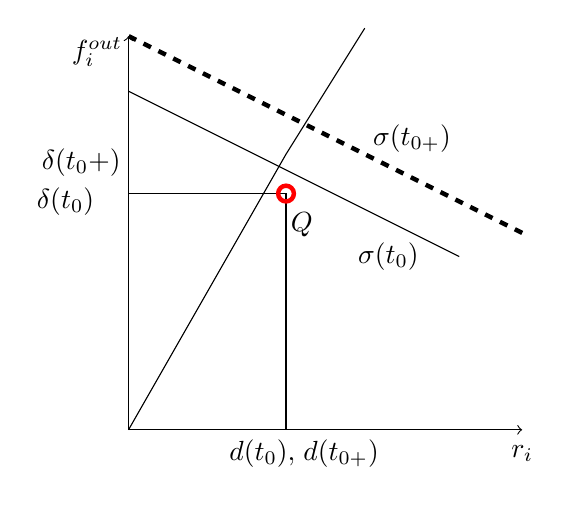
\begin{tikzpicture}
	\draw[<->] (0,5) -- (0,0) --(5,0);
	\draw (0,0) rectangle (2,3);
	%\draw [dashed](0,0) rectangle (2.3,3.3);
	%\draw [dashed, ultra thick](0,3.3) -- (2.3,3.3);
	%\draw [dashed, ultra thick](2.3,3.3) -- (2.3,0);
	\draw (4.2,2.2) -- (2.2,3.2)--(0,4.3);
	\draw [dashed, ultra thick](5,2.5) -- (2,4)--(0,5);
	%\draw [dashed](2,3) -- (2.3,3);
	%\draw [dashed](2,3) -- (2,3.3);
	%\draw[fill=gray] (0,0)--(0,3) to (0,0) -- (2,0) to (2,0)--(2,1.5) to (2, 1.5)--(1,3) to (0.58,3)--(0,3) ;
	\draw (0,0) -- (2,3.5)--(3,5.1);
	\draw[ultra thick, red](2,3) circle (0.1);
	\node (below) at (5,-0.3) {$r_i$};
	\node (below) at (1.7,-0.3) {$d(t_0),$};
	\node (below) at (2.7,-0.3) {$d(t_{0+})$};
	\node (left) at (-0.4,4.8) {$f_i^{\text{out}}$};
	\node (left) at (-0.8,2.9) {$\delta(t_0)$};
	\node (above) at (3.6,3.7) {$\sigma(t_{0+})$};
	\node (above) at (3.3,2.2) {$\sigma(t_{0})$};
	\node (left) at (-0.6,3.4) {$\delta(t_0+)$};
	%\node (right) at (3.5,1.5) {$\hat{\gamma}_3=\gamma_1+\gamma_2$};
%	\node (above) at (1,1.5) {$\Omega$};
	%\node (right) at (3.2,4) {$\gamma_2=\frac{P}{1-P}\gamma_1$};
	\node (below) at (2.2,2.6) {$Q$};
\end{tikzpicture}